% +---------------------------------------------------------------+
% Indicates which master document to compile
% TeXstudio
% !TeX master = ../tb_report.tex
%
% TeXShop
% !TEX root = ../tb_report.tex

\chapter{Example of Chapter}

\lipsum[1]


\section{Writing Mathematical Expressions}
\todo{example of todo}

Here is an inline math example: $3^2 / 4^3$.

Or on a separate line:

$$ \frac{3 x_a}{ y_b^2 +4}$$

\section{Inserting Images}

Here is how to insert an image.

\begin{figure}
	\centering
	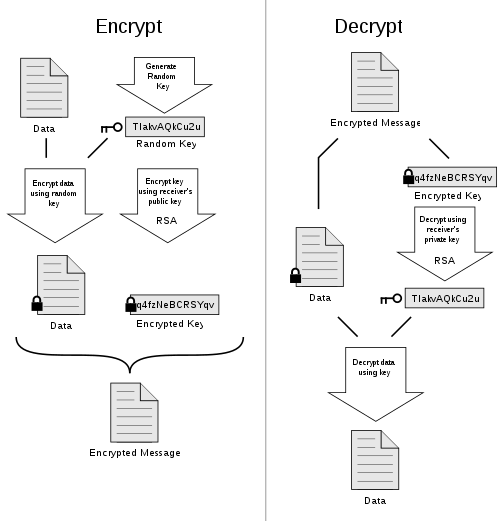
\includegraphics[width=8cm]{images/PGP_101.png}
	\caption{PGP Diagram}
	\label{fig:pgp}
\end{figure}


\section{Creating and Citing Bibliographic References}
\todo{improve my bibliography}

This is an example of citing a book by Pasini~\cite{pasini2015}.

But also a website, Black Alps 2019~\cite{BA19}!


\section{Creating References to Other Parts of the Document}

You can also add a reference to Section~\ref{sec:shell}.

You can also add a reference to the introduction, Chapter~\ref{ch:intro}.

As shown in Figure~\ref{fig:pgp}, you can reference a figure.


\section{Displaying a Simple Command or Bash}

Use the command \com{com}.

Example: Testing a bash shell command \com{ls}:

Use the environment \com{shellcmd}.

\begin{shellcmd}
	$> ls -al test_underscore $$* "hello"
\end{shellcmd}
Blah blah


\section{Displaying a Shell Command}
\label{sec:shell}

Here is how to format a SHELL command.

Use the \com{listingsbox} environment.
\begin{description}
	\item[1st parameter:] the type of shell, here "console"
	\item[2nd parameter:] the name to give to the box
\end{description}

\begin{listingsbox}{console}{Example of shell command with output}
	root@kali:~$ bunzip2 data-decrypted.bin
	bunzip2: Can't guess original name for data-decrypted.bin -- using
	data-decrypted.bin.out
\end{listingsbox}


\section{Including Code in LaTeX}

Use the \com{sourcebox} environment.
\begin{description}
	\item[1st parameter:] the language, here "c"
	\item[2nd parameter:] the name to give to the box
\end{description}

\begin{sourcebox}{c}{Example C code}
	#include <stdio.h>

	int main(int argc, char* argv[])
	{
			printf("Hello World!\n");
			return 0;
	}
\end{sourcebox}



\section{Including Code from an External Source File}

Use the command \com{inputsourcecode}.
\begin{description}
	\item[1st parameter:] the language, here "c"
	\item[2nd parameter:] the source file name, "\path{source_code/example.c}"\\ Also an example of the \com{path} command.
	\item[3rd parameter:] the name to give to the box
\end{description}


%% Include source code from an external file
%% 1st parameter: code language
%% 2nd parameter: path to the source file
%% 3rd parameter: title of the box
\inputsourcecode{c}{source_code/example.c}{example.c}

Same example, but specifying lines 4 to 8:
\inputsourcecode[firstline=4,lastline=8]{c}{source_code/example.c}{example.c}